\section{Odometry}\label{sec:visual-odometry}
As introduced in \S1.2, the problem of odometry is about the estimation of the change in a robot's pose over time.

The odometry, also known as self-localization, can be classified in different ways, in \S2.2.1 there is a more detailed description of the different types of odometry.

\subsection{Taxonomy}\label{subsec:tassonomy}
There different types of odometry, which based on the classification of ~\cite{vo_state_of_art} can be divided into two main categories: \textit{GNSS available} and \textit{GNSS not available}.
\begin{figure}[H]
    \centering
    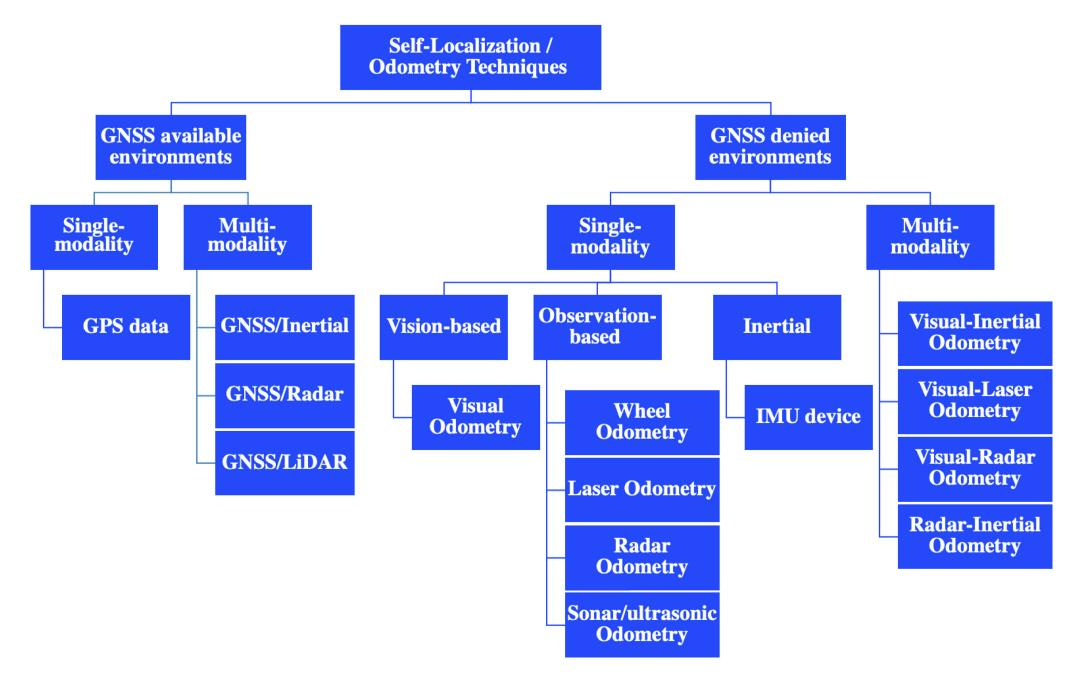
\includegraphics[width=\textwidth]{images/2_2_taxonomy_odometry}
    \caption{Taxonomy of odometry techniques}\label{fig:odometry-taxonomy}
\end{figure}

\subsection{Reference systems}\label{subsec:reference-systems}
To tackle the problem of odometry, we need as to choose the representation system to adopt.
There are many way of representing the pose of the camera or the robot, but the most common are the \textit{Euler angles} and the \textit{quaternions} and \textit{rotation matrix} combined with \textit{translation matrix}.
% TODO add how to translate the poses origin.

\subsection[Reference systems conversion]{Reference systems conversion}\label{subsec:reference-systems-conversion}

\subsection{State of the art}\label{subsec:state-of-the-art}

\subsection[Metrics]{ATE and RTE}\label{subsec:ate-and-rte}
As presented in~\cite{measuring_robustness_of_visual_slam}, we can measure the global consistency of the trajectory by comparing the absolute distances between estimated and ground truth trajectory.
As both trajectories can be specified in arbitrary coordinate frames, they first need to be aligned.
Then, we should define the absolute trajectory error matrix at time $i$ as:
\begin{equation}
    \label{eq:ate-error-matrix}
    E_i \coloneq Q_i^{-1} SP_i
\end{equation}
Where S is the rigid-body transformation found by Horn Method (~\cite{horn_method}).
Then, the ATE is defined as the root-mean-square error from error matrices:
\begin{equation}
    ATE_{rmse} = (\frac{1}{n} \sum_{i=1}^{n} ||E_i||^2)^{1/2}
    \label{eq:ate-rmse}
\end{equation}
The relative pose error measure is the local accuracy of the trajectory over a fixed time interval $\Delta$.
Therefore, the RTE corresponds to the drift of the trajectory which is in particular useful for the evaluation of visual odometry systems.
The RTE is defined as follows:
\begin{equation}
    F_i^{\Delta} \coloneq (Q_i^{-1} Q_{i+\Delta})^{-1} (P_i^{-1} P_{i+\Delta})
    \label{eq:rte}
\end{equation}
from a sequence of $n$ camera poses we obtain  $m = n - \Delta$ individual relative pose error matrices along the sequence.
The RPE is usually divided into translation component and rotation component.
Similarly to ATE, we can compute the root-mean-square error over all time indices for RPE translation error:
\begin{equation}
    RPE_{trans}^{i, \Delta} \coloneq (\frac{1}{m} \sum_{i=1}^m ||trans(F_i)||^2)^{½}
    \label{eq:rpe-trans}
\end{equation}
And for the rotation component we use mean error approach:
\begin{equation}
RPE_{trans}^{i, \Delta} \coloneq \frac{1}{m} \sum_{i=1}^m \angle (rot(F_i^\Delta))
\label{eq:equation-rpe-trans}
\end{equation}